% % -*- coding:utf-8 -*-
\documentclass[aspectratio=169,10pt]{beamer}
\nonstopmode

\usepackage{pifont}
\usepackage{subcaption}
\usepackage{graphicx}
\usepackage{enumitem}
\usepackage{caption}
\usepackage{tikz}
\usetikzlibrary{positioning}

\usepackage[style=authoryear,backend=biber]{biblatex}
\addbibresource{bibliography.bib}

\captionsetup{skip=4pt}
% color palette
\definecolor{tu01}{HTML}{84B818}
\definecolor{tu02}{HTML}{D18B12}
\definecolor{tu03}{HTML}{1BB5B5}
\definecolor{tu04}{HTML}{F85A3E}
\definecolor{tu05}{HTML}{4B6CFC}
\definecolor{tu06}{HTML}{E3B505}
\definecolor{tu07}{HTML}{AF331D}
\definecolor{tu08}{HTML}{000000}
\definecolor{tu09}{HTML}{AAAAAA}
\definecolor{tu10}{HTML}{444444}
\definecolor{tu11}{HTML}{84B818}

% mixed and light colors
\colorlet{tu01light}{tu01!33}
\colorlet{tu02light}{tu02!33}
\colorlet{tu03light}{tu03!33}
\colorlet{tu04light}{tu04!33}
\colorlet{tu05light}{tu05!33}
\colorlet{tu06light}{tu06!33}
\colorlet{tu07light}{tu07!33}
\colorlet{tu08light}{tu08!33}
\colorlet{tu09light}{tu09!33}
\colorlet{tu10light}{tu10!33}
\colorlet{tu11light}{tu11!33}

\colorlet{tu01midlight}{tu01!50}
\colorlet{tu02midlight}{tu02!50}
\colorlet{tu03midlight}{tu03!50}
\colorlet{tu04midlight}{tu04!50}
\colorlet{tu05midlight}{tu05!50}
\colorlet{tu06midlight}{tu06!50}
\colorlet{tu07midlight}{tu07!50}
\colorlet{tu08midlight}{tu08!50}
\colorlet{tu09midlight}{tu09!50}
\colorlet{tu10midlight}{tu10!50}
\colorlet{tu11midlight}{tu11!50}

\colorlet{tu01dark}{tu01!80!black}
\colorlet{tu02dark}{tu02!80!black}
\colorlet{tu03dark}{tu03!80!black}
\colorlet{tu04dark}{tu04!80!black}
\colorlet{tu05dark}{tu05!80!black}
\colorlet{tu06dark}{tu06!80!black}
\colorlet{tu07dark}{tu07!80!black}
\colorlet{tu08dark}{tu08!80!black}
\colorlet{tu09dark}{tu09!80!black}
\colorlet{tu10dark}{tu10!80!black}
\colorlet{tu11dark}{tu11!80!black}

\colorlet{lightgray}{gray!25}
\colorlet{midlightgray}{gray!50}
\colorlet{anthracite}{black!85}

% aliases
\colorlet{tudo}{tu01}
\colorlet{tuorange}{tu02}
\colorlet{tudolight}{tu01light}

\usetheme[progressbar=frametitle]{metropolis}
\metroset{progressbar=none}
\newcommand{\themename}{\textbf{\textsc{metropolis}}\xspace}
\newcounter{mainframenumber}
\newcommand{\backupbegin}{
  \setcounter{mainframenumber}{\value{framenumber}}
}



\usepackage{xcolor}
\setbeamertemplate{navigation symbols}{}
\setbeamercolor{background canvas}{bg=white}

% Custom footline with frame numbers on the left and navigation symbols on the right
\setbeamertemplate{footline}{
  \leavevmode%
  \hbox{%
    \begin{beamercolorbox}[wd=.1\paperwidth,ht=2.5ex,dp=1.125ex,leftskip=1em,rightskip=1em]{author in head/foot}%
      \usebeamerfont{footline} \insertframenumber{} / 22
    \end{beamercolorbox}%
    \hfill
    \begin{beamercolorbox}[wd=.9\paperwidth,ht=2.5ex,dp=1.125ex,leftskip=1em,rightskip=1em]{author in head/foot}%
      \usebeamerfont{footline} %\insertnavigation{2cm}
    \end{beamercolorbox}%
  }%
  \vskip0pt%
}

%%%%%%%%%%%%%%%%%%%%%%%%%%%%%%%%%%%%%%%%%%%%%%%%%%%%%% PRESENTATION START %%%%%%%%%%%%%%%%%%%%%%%%%%%%%%%%%%%%%%%%%%%%%%%%%

\titlegraphic{
  \hfill{
\includegraphics[height=1.25cm]{figures/logoUnimi.png}}
}
\title{Development of an open-source calibration framework\\ for superconducting qubits}
\subtitle{Master's degree in Physics}
\author{Elisa Stabilini}
\institute{Università degli Studi di Milano - Department of Physics}
\date{July 4th 2025}

\begin{document}

\maketitle

\begin{frame}{Table of contents}
    \setbeamertemplate{section in toc}[sections numbered]
    \setbeamertemplate{subsection in toc}[subsections numbered]  
    \tableofcontents[hideallsubsections]
\end{frame}

\begin{frame}{Quantum Computing, what for?}
  \begin{columns}
    \begin{column}{0.5\textwidth}
      \begin{itemize}[label=\textbullet]
        \small
        \item<2-> Simulation of quantum system: classical computers can not efficiently simulate quantum staes. Classical computers can usally simulate a $\sim 30$ qubits  
        \item<3-> Optimization and modeling (eg. direct annealing, adiabatic evolutions, QAOA) with applications in finance, traffic, weather... 
        \item<4-> Gate-based circuits (eg. Shor, Grover, Deutsch)
        \item<5-> AI-inspired algorithms (VQE, autoencoders, classifiers ...)
      \end{itemize}
      \end{column}
      \begin{column}{0.5\textwidth}
        \begin{center}
            \onslide<1->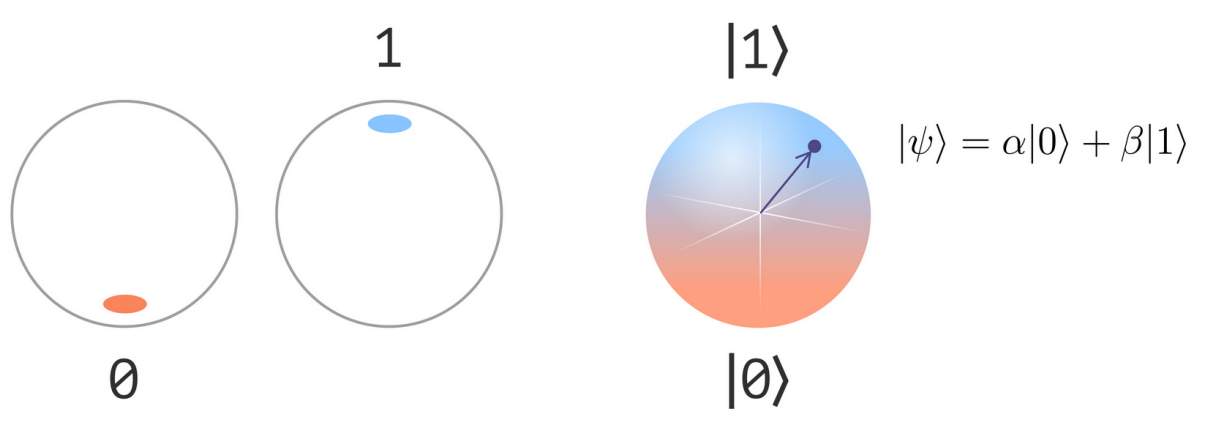
\includegraphics[width=0.75\textwidth]{figures/BlochSphere.png}\\
            \vspace*{1.75em}
            \onslide<4->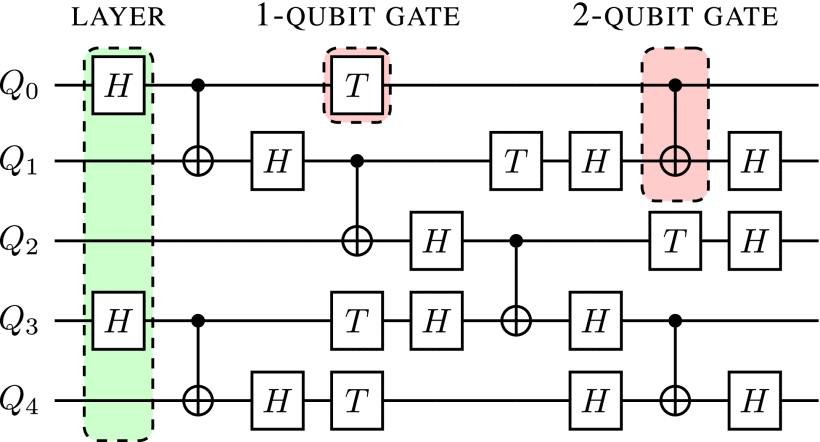
\includegraphics[width=0.75\textwidth]{figures/circuit.png}\\
            \onslide<4->{\tiny DOI: 10.1109/TQE.2021.3053921}
        \end{center}
      \end{column}
  \end{columns}
\end{frame}



\section{Superconducting qubits}

\begin{frame}{Artificial atoms \hfill{\small[arXiv:cond-mat/0703002]}}
  \begin{columns}
    \begin{column}{0.6\textwidth}
      \centering
      \begin{itemize}
        \item<1-> Qubit: two level quantum system
        \hspace{10 mm}
        \item<2-> Superconducting qubits: use Josephson Junctions\\ to build anharmonic oscillators
      \end{itemize}
      \begin{figure}
        \centering
        \onslide<2->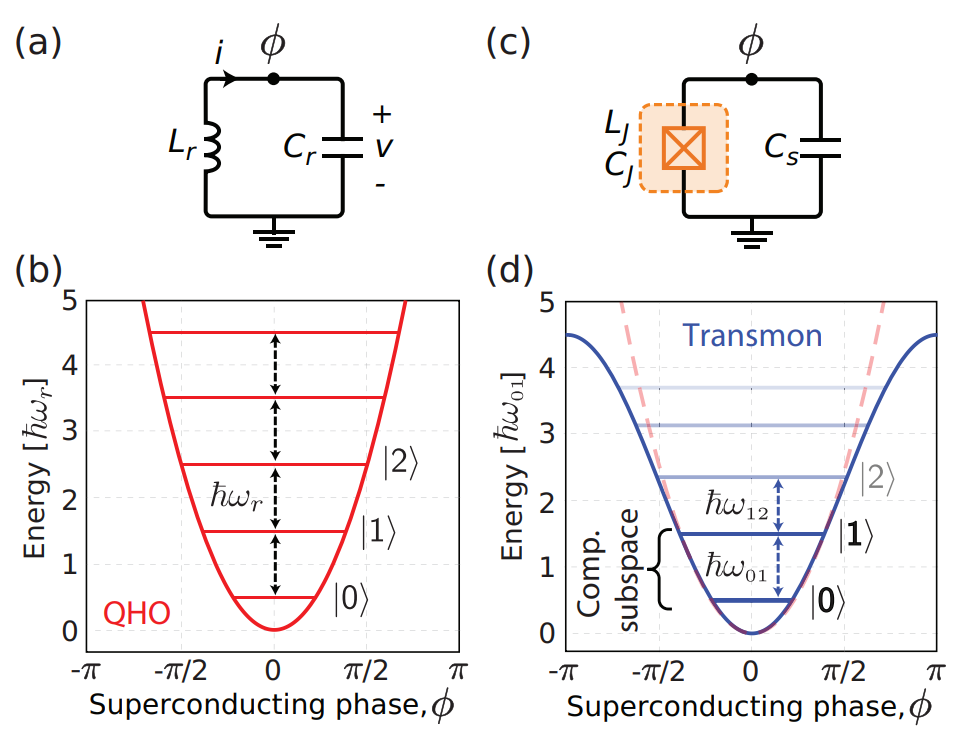
\includegraphics[height=0.5\textheight]{figures/Transmon.png}\\
        \onslide<2->{\tiny DOI: 10.1109/MAP.2022.3176593}      
      \end{figure}
    \end{column}
    \begin{column}{0.6\textwidth}
      \centering
      \onslide<2->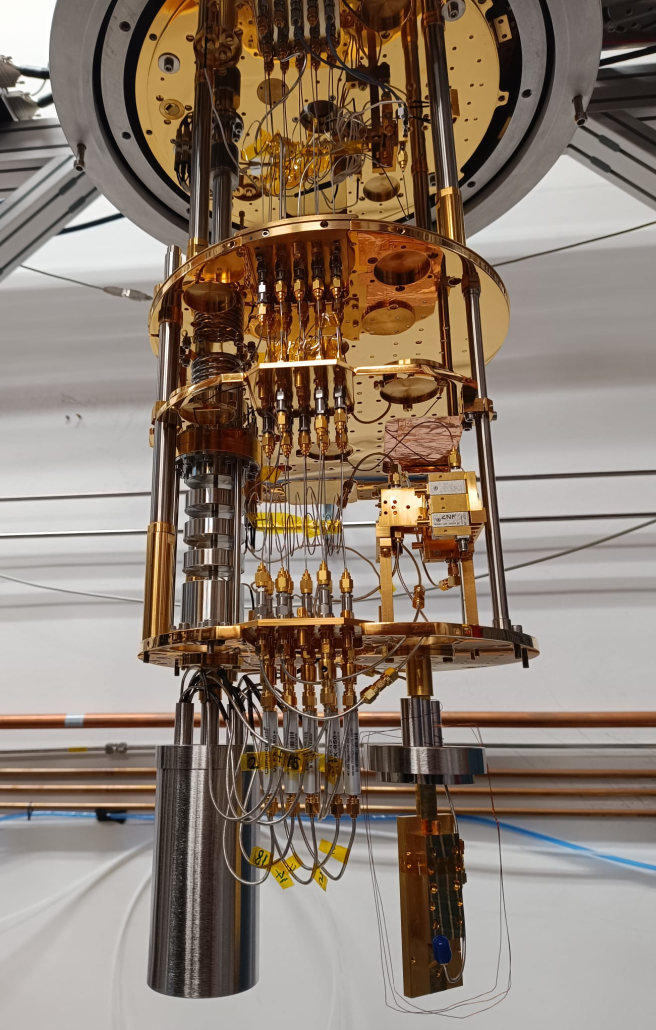
\includegraphics[width=0.5\textwidth]{figures/cryostat.png}
    \end{column}
  \end{columns}
\end{frame}

\begin{frame}{Qubit control \hfill{\small[arXiv:2403.04383]}}

  \begin{columns}
    \begin{column}{0.45\textwidth}
      \small

      \onslide<2->{Microwave pulse applied to the qubit
      \begin{equation*}
        V_d(t) = A\varepsilon(t)\sin{(\omega_d t + \alpha)};
      \end{equation*}\\
      \vspace{1.5em}}

      \onslide<3->{Qubit - electric field Hamiltonian (RWA)
      \begin{equation*}
        \hat{H} = -\frac{\hbar (\omega_q - \omega_d)}{2} \hat{\sigma}_z + \frac{\hbar \Omega}{2} \varepsilon(t) \left( \hat{\sigma}_x \cos \alpha + \hat{\sigma}_y \sin \alpha \right);
      \end{equation*}\\
      \vspace{1.5em}}


      \onslide<4->{Qubit evolution under microwave pulse:
      \begin{equation*}
        R_{\hat{n}(\alpha)}(\theta) = e^{-\frac{i}{2} \hat{n}(\alpha) \cdot \vec{\sigma} \theta} = e^{-\frac{i}{2} (\hat{\sigma}_x \cos \alpha + \hat{\sigma}_y \sin \alpha) \theta};
      \end{equation*}
      where $\theta = \Omega\int_{0}^{+\infty}\varepsilon(t')dt'$.}

    \end{column}
    \onslide<1->\begin{column}{0.55\textwidth}
      \centering
      \begin{figure}
        \centering
        \vspace{2mm}
        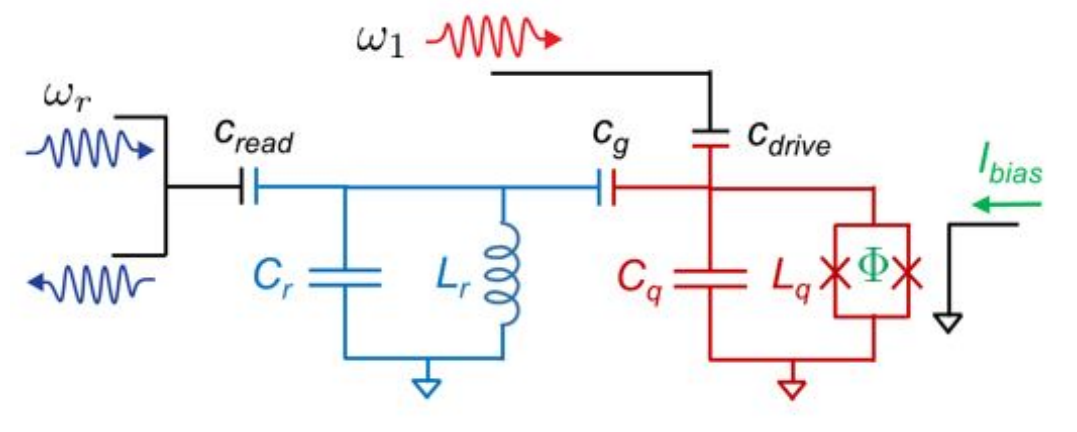
\includegraphics[width=0.8\textwidth]{figures/TransmonCircuit.png}\\
        \vspace{1.5em}
        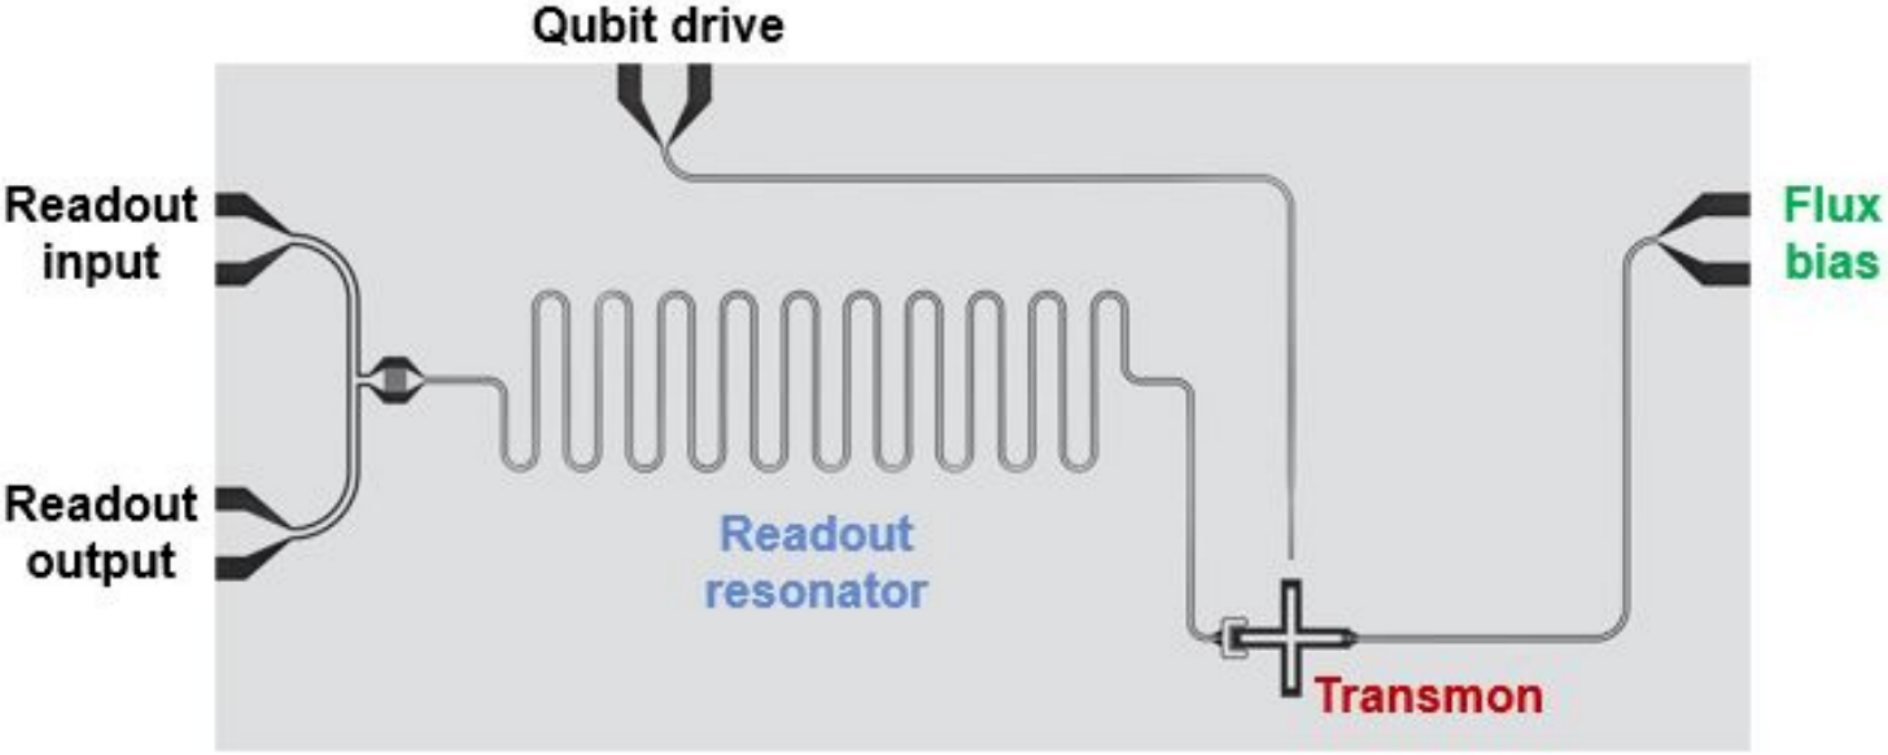
\includegraphics[width=0.8\textwidth]{figures/TransmonBoard.png}\\
        {\tiny DOI: 10.1109/MAP.2022.3176593}
      \end{figure}
    \end{column}
  \end{columns}   


\end{frame}

\begin{frame}{State readout \hfill{\small[arXiv:cond-mat/0407325]}}
  \begin{columns}
    \begin{column}{0.35\textwidth}
      \onslide<1->{Qubit - resonator Hamiltonian:
      \begin{equation*}
        \hat{H} = \hbar\omega_r\hat{a}\hat{a}^\dagger - \frac{\hbar\omega_{01}}{2}\hat{\sigma}_z + \hbar g(\hat{\sigma}^+\hat{a}+\hat{\sigma}^-\hat{a}^\dagger);
      \end{equation*}\\}
      \vspace{1.5em}
      \onslide<2->{Dispersive regime ($g \ll \omega_q - \omega_r$):
      \begin{equation*}
        \hat{H}_{disp} = \hbar(\omega_r - \chi\hat{\sigma}_z)\hat{a}^\dagger\hat{a} - \frac{\hbar}{2}(\omega_{01}+\chi)\hat{\sigma}_z;
      \end{equation*}
      dispersive shift: $\chi = \frac{g^2}{\Delta},$ \hfill $\Delta = \omega_q - \omega_r$.}
    \end{column}
    \begin{column}{0.65\textwidth}
      \centering
      \onslide<2->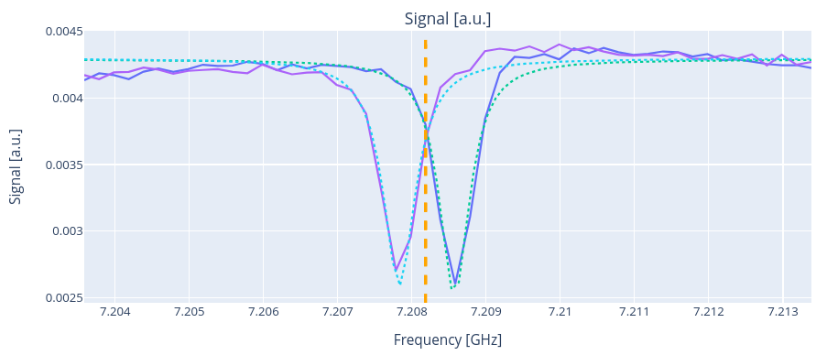
\includegraphics[width=0.75\textwidth]{figures/disp_sihft.png}
      \hspace{5mm}
      \onslide<3->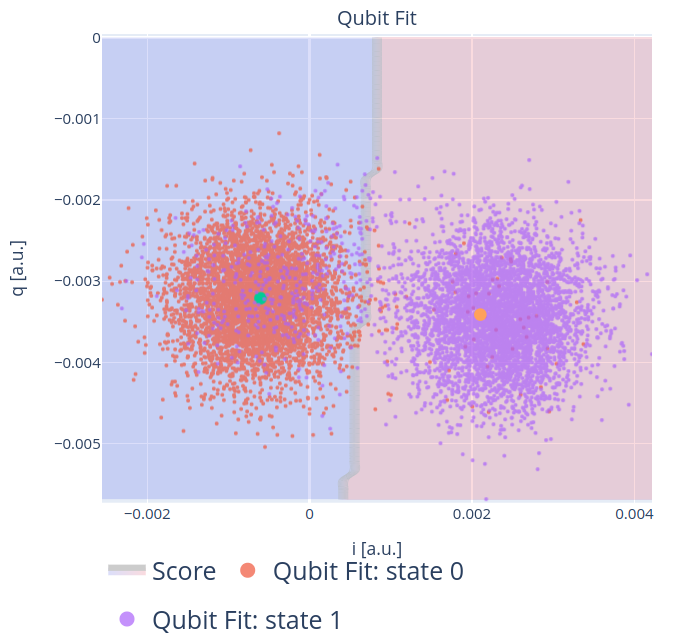
\includegraphics[height=0.48\textwidth]{figures/classification.png}
    \end{column}
  \end{columns}
\end{frame}



\section{Quantum Middleware}

\begin{frame}{Superconducting qubit calibration}
  \begin{itemize}
    \item<1-> Circuit: sequence of quantum gates applied to qubits to perform a computation.
    \item<2-> Gates: abstract unitary operations (logical or native).
    \item<3-> Pulses: physical signal (control field) implementing a gate.
  \end{itemize}
\vspace{0.75em}
  \resizebox{\textwidth}{!}{
  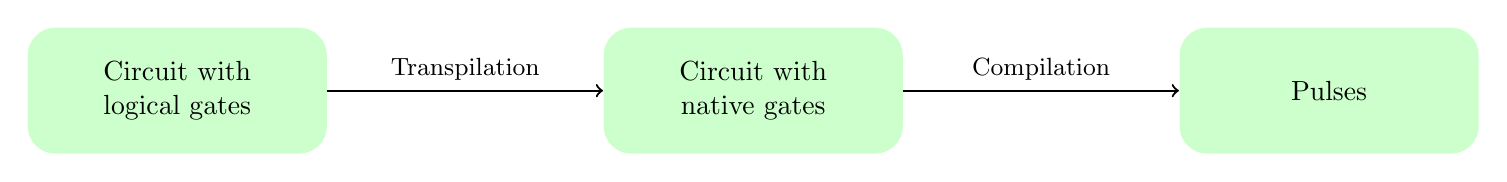
\begin{tikzpicture}[
      box/.style={rectangle, rounded corners=10pt, fill=green!20, minimum width=3.8cm, minimum height=1.6cm, align=center},
      arrow/.style={->, thick},
      label/.style={font=\small, midway, above}
    ]

    \onslide<1->{\node[box] (logical) {Circuit with\\logical gates};}
    \onslide<2->{\node[box, right=3.5cm of logical] (native) {Circuit with\\native gates};}
    \onslide<3->{\node[box, right=3.5cm of native] (pulses) {Pulses};}

    \onslide<2->{\draw[arrow] (logical) -- node[label] {Transpilation} (native);}
    \onslide<3->{\draw[arrow] (native) -- node[label] {Compilation} (pulses);}

  \end{tikzpicture}
  }
  \vspace{0.75em}
  \begin{itemize}
    \item<2-> We need to calibrate \textit{only} native gates.
    \item<2-> Native single qubit gates on superconducting qubits: $R_X(\pi)$, $R_X(\frac{\pi}{2})$, $R_Z(\theta)$.
    \item<3-> For each pulse we calibrate frequency, duration, power, shape.
  \end{itemize}
\end{frame}

\begin{frame}[t,fragile]{Qibo framework \hfill{\small[arXiv:2308.06313]}}
  \setlength{\topskip}{0pt}
  \setlength{\textheight}{\paperheight}
  \vspace*{-0.5cm}
  \begin{center}
      {\fontsize{10pt}{0pt}\selectfont Qibo: a modular and open-source framework for quantum computing, control and calibration.}\\
      \vspace*{0.5em}
      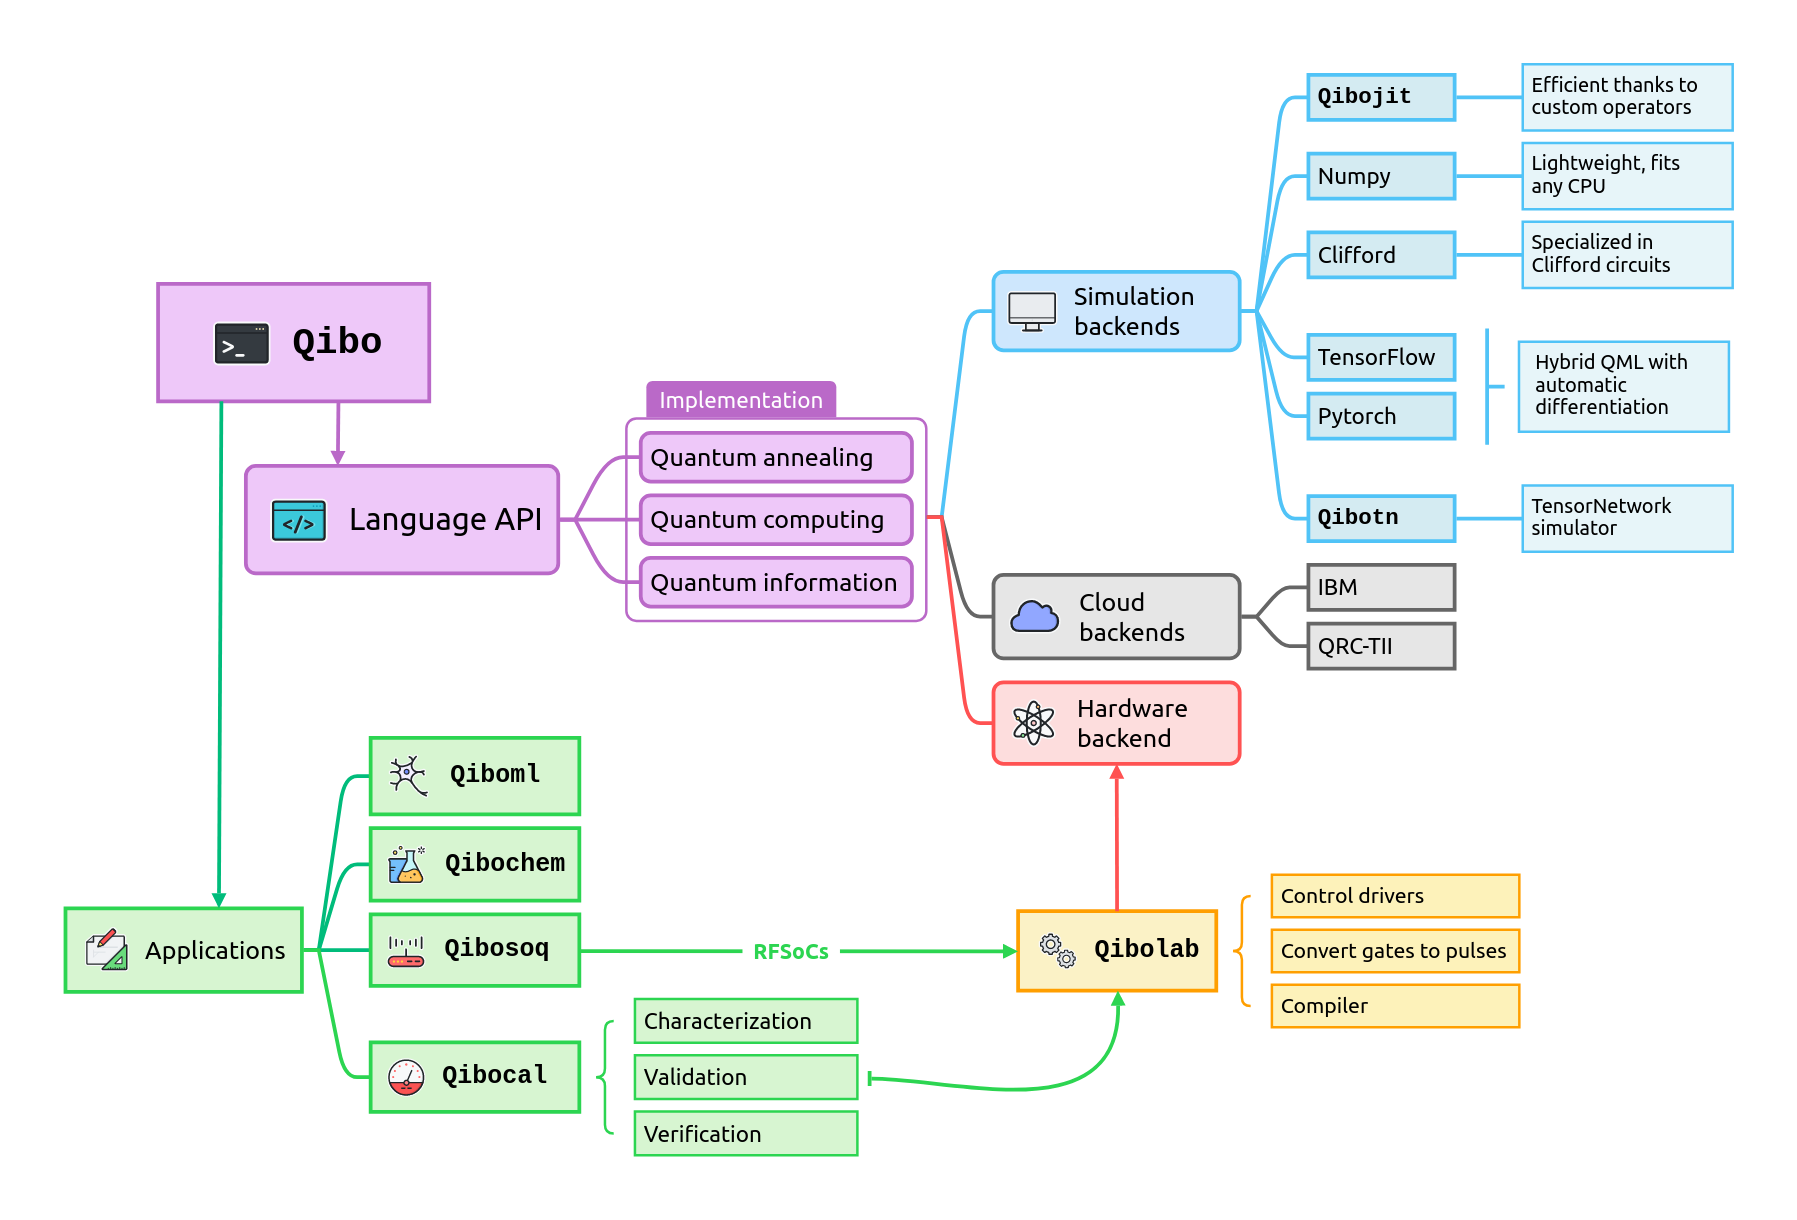
\includegraphics[height=0.7\paperheight]{figures/qibo_ecosystem.png}\\
      \vfill
      {\fontsize{8pt}{0pt}\selectfont \url{https://qibo.science/}}
  \end{center}
\end{frame}



\section{Average Clifford gate fidelity optimization}

\begin{frame}[t,fragile]{Randomized Benchmarking \hfill{\small[arXiv:0707.0963v1]}}

  \begin{itemize}
    \item<1-> Randomized benchmarking estimates average gate fidelity by applying random sequences of Clifford gates followed by an inverting gate.
    \item<2-> Randomization with Clifford gates provides a depolarized noise channel: $\rho \rightarrow d \frac{\mathbb{I}}{2} + (1-d)\rho$.
  \end{itemize}

  \vspace{3mm}
  \onslide<3->{Randomized Benchmarking protocol:
  {\setbeamertemplate{enumerate items}[default]
   \begin{enumerate}[leftmargin=*, label=\arabic*.]
     \item Initialize the system in the ground state
     \item For each sequence length $m$ draw a sequence of Clifford group elements
     \item Calculate the inverse gate 
     \item Measure complete sequence
     \item Repeat the process for multiple sequences of the same length while varying the length
  \end{enumerate}}}
\end{frame}

\begin{frame}[t,fragile]{Randomized Benchmarking \hfill{\small[arXiv:0707.0963v1]}}
  \begin{itemize}
    \item<1-> The survival probability decays exponentially with the number of Clifford gates $F(m) = Ap^m + B$ where $1-p$ is the depolarization rate.\\
    \item<2-> From $p$ we can extract the average error per Clifford gate.\\
  \end{itemize}

  \begin{center}
    \vspace{0.5em}
    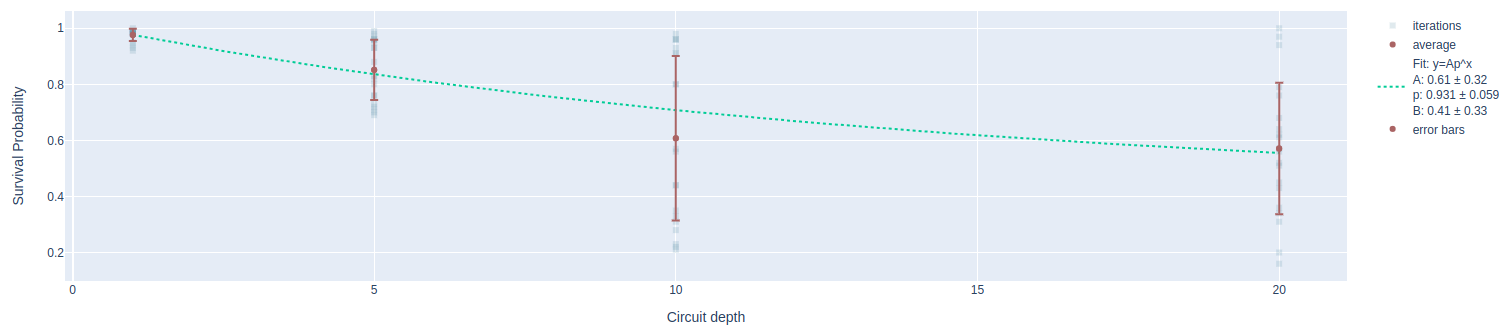
\includegraphics[width=\textwidth]{figures/rb.png}\\
    \vspace{1.25em}
    \onslide<3->{Can we optimize the average Clifford gate fidelity to automate $R_X(\pi)$ gate recalibration?}
  \end{center}
\end{frame}

\begin{frame}[t,fragile]{RB optimization \hfill{\small[arXiv:1403.0035]}}
  \begin{center}
    \onslide<1->Test closed-loop optimization with modern optimization libraries.\\
  \end{center}
  \vspace*{1.25em}
  \resizebox{\textwidth}{!}{
  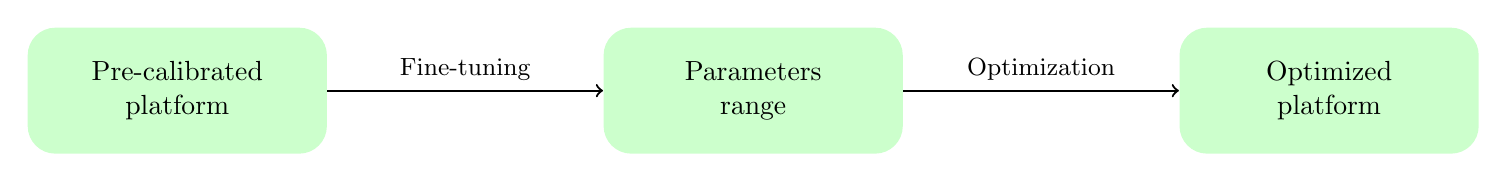
\begin{tikzpicture}[
      box/.style={rectangle, rounded corners=10pt, fill=green!20, minimum width=3.8cm, minimum height=1.6cm, align=center},
      arrow/.style={->, thick},
      label/.style={font=\small, midway, above}
    ]

    \onslide<2->{\node[box] (logical) {Pre-calibrated\\platform};}
    \onslide<3->{\node[box, right=3.5cm of logical] (native) {Parameters\\range};}
    \onslide<4->{\node[box, right=3.5cm of native] (pulses) {Optimized\\platform};}

    \onslide<3->{\draw[arrow] (logical) -- node[label] {Fine-tuning} (native);}
    \onslide<4->{\draw[arrow] (native) -- node[label] {Optimization} (pulses);}

  \end{tikzpicture}
  }

  \vspace{1.25em}
  Optimization parameters:
  \begin{itemize}
    \item Pulse amplitude
    \item Pulse frequency
    \item Pulse shape (through $\beta$ DRAG parameter)
  \end{itemize}
\end{frame}


\begin{frame}[t,fragile]{Average Clifford gate Fidelity}
    \vbox to \textheight{ 
    \vspace{1em}
    \begin{minipage}[t]{\textwidth}
      \centering
      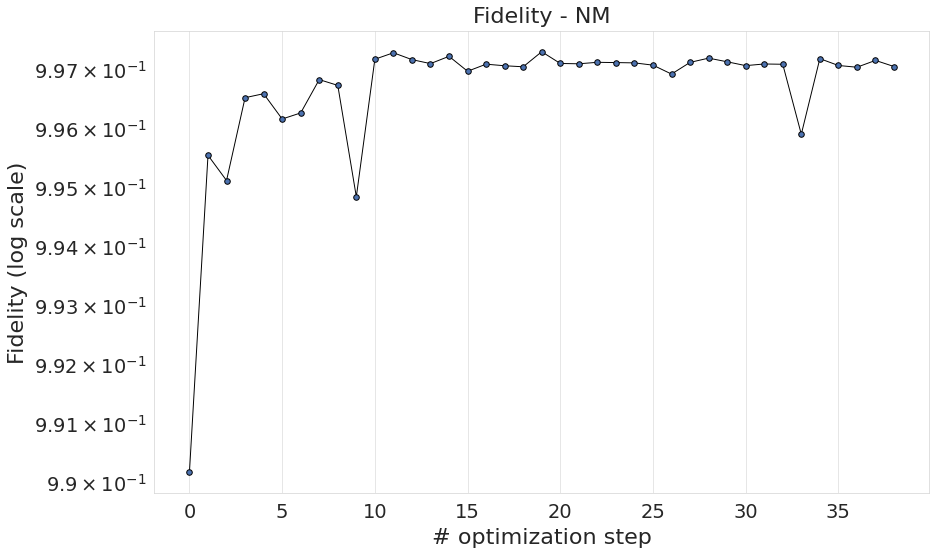
\includegraphics[height=0.35\textheight]{figures/NM_fidelity.png}
      \hspace{10mm}
      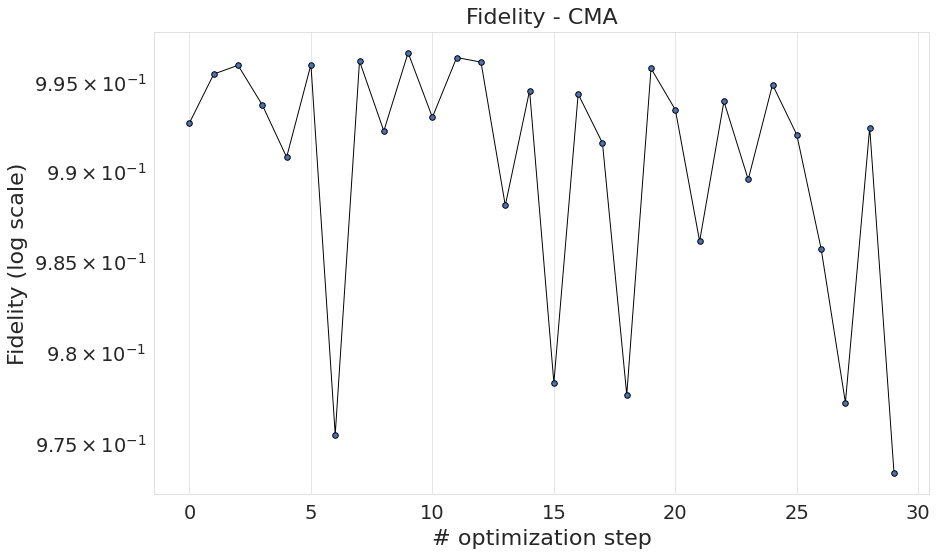
\includegraphics[height=0.35\textheight]{figures/CMA_fidelity.png}
    \end{minipage}
    \vspace{0.5em}
    \begin{minipage}[b]{\textwidth}
      \centering
      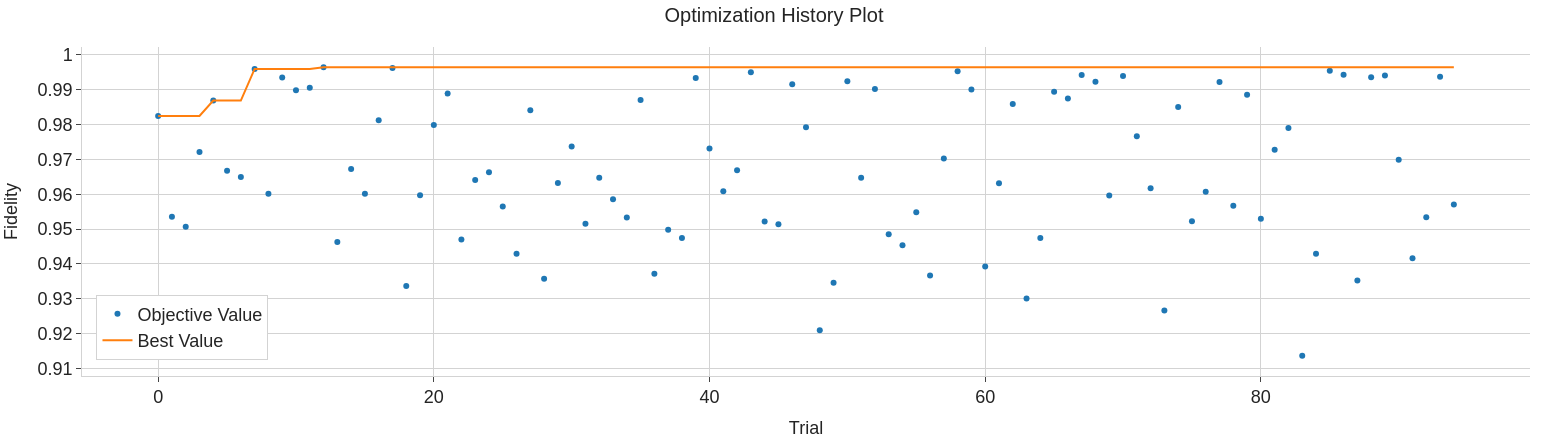
\includegraphics[width=0.85\textwidth]{figures/optuna.png}
    \end{minipage}
    \vspace{1em}
  }
\end{frame}

\begin{frame}[t,fragile]{Parameters evolution}
  \begin{figure}
    \begin{subfigure}[t]{0.315\textwidth}
      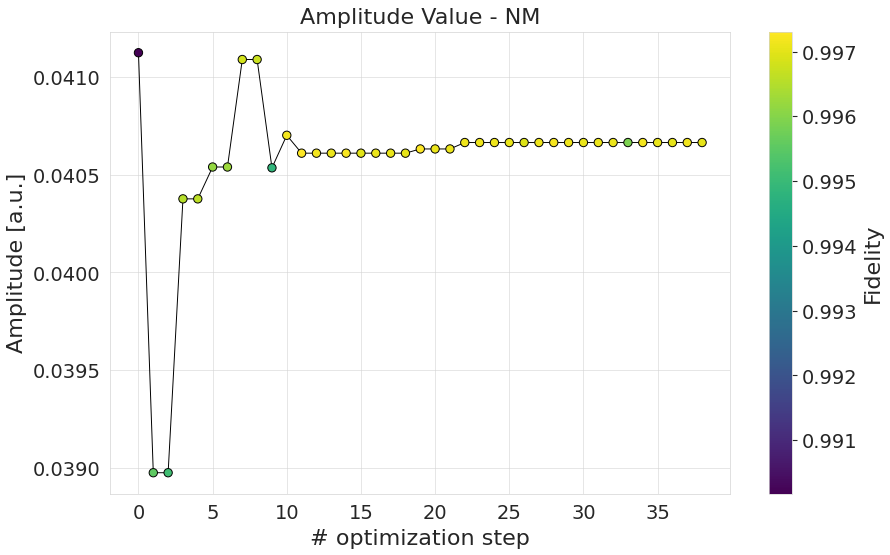
\includegraphics[width=\textwidth]{figures/NM_amplitude.png}
    \end{subfigure}
        \begin{subfigure}[t]{0.315\textwidth}
      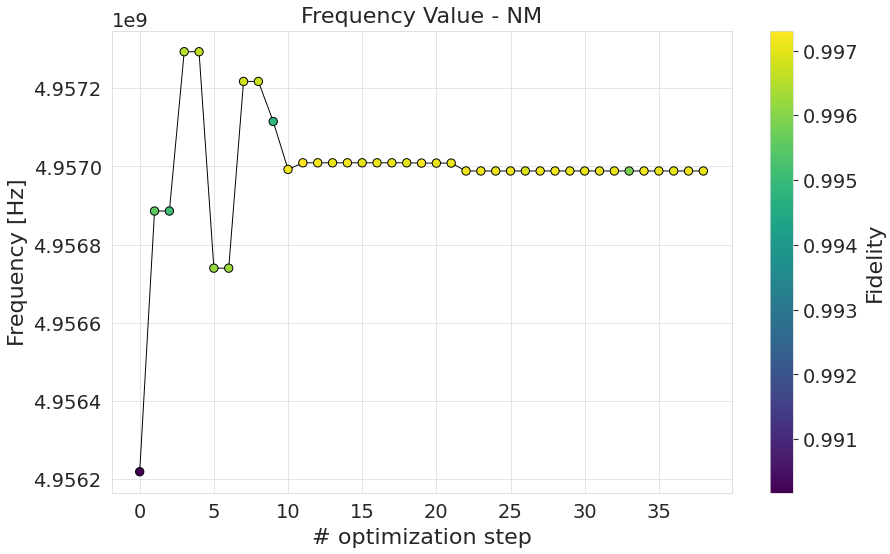
\includegraphics[width=\textwidth]{figures/NM_frequency.png}
    \end{subfigure}
        \begin{subfigure}[t]{0.315\textwidth}
      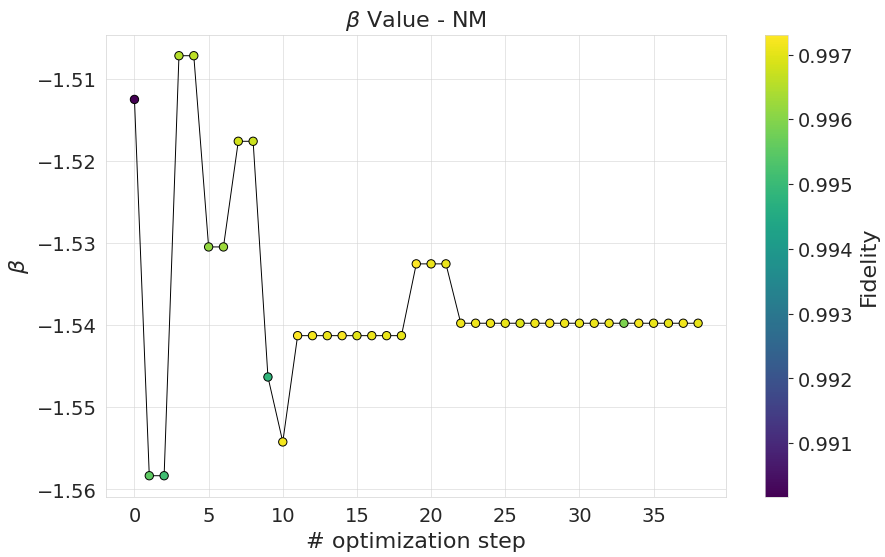
\includegraphics[width=\textwidth]{figures/NM_beta.png}
    \end{subfigure}

  \end{figure}
    \begin{figure}
    \begin{subfigure}[t]{0.315\textwidth}
      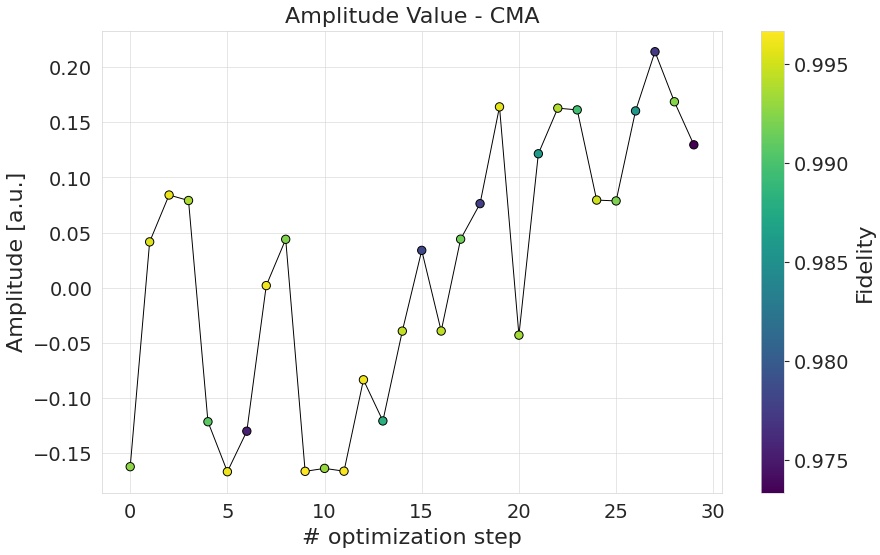
\includegraphics[width=\textwidth]{figures/CMA_amplitude.png}
    \end{subfigure}
        \begin{subfigure}[t]{0.315\textwidth}
      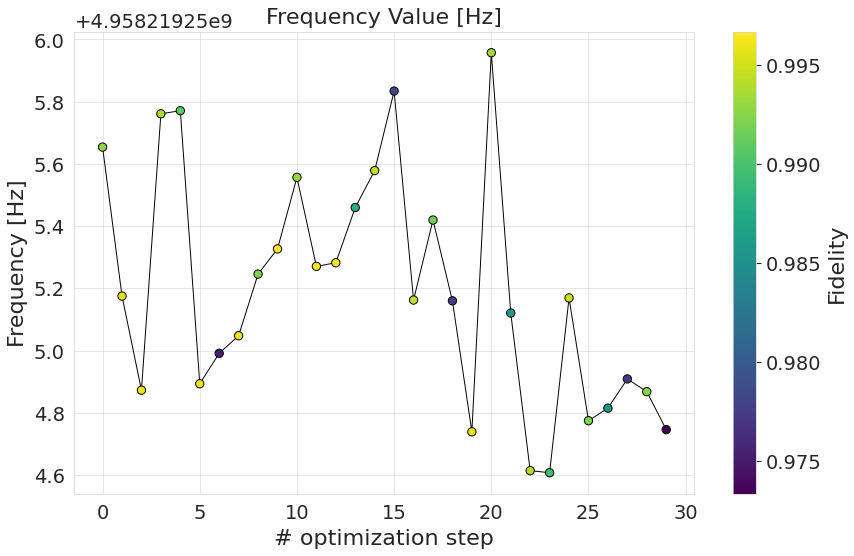
\includegraphics[width=\textwidth]{figures/CMA_frequency.png}
    \end{subfigure}
        \begin{subfigure}[t]{0.315\textwidth}
      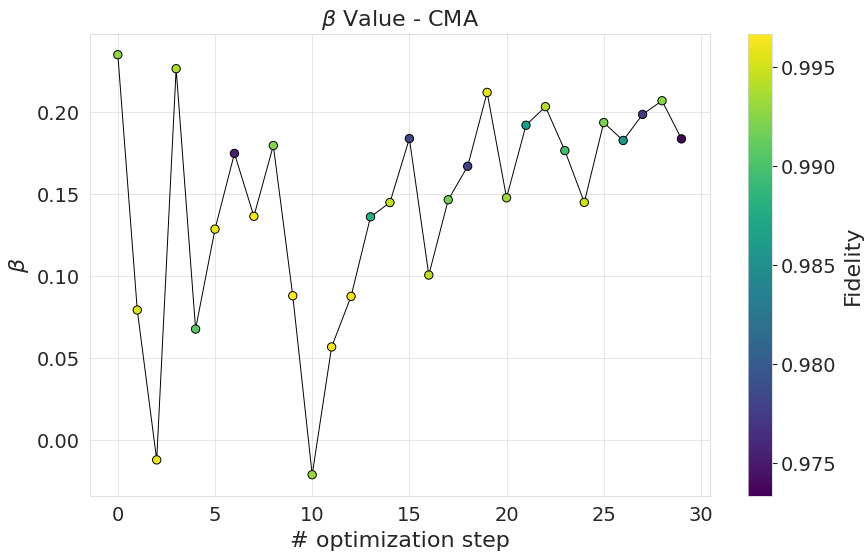
\includegraphics[width=\textwidth]{figures/CMA_beta.png}
    \end{subfigure}
  \end{figure}
\end{frame}




\section{New features in Qibo}

\subsection{Native RX90}

\begin{frame}{Improving Qubit Control for Calibration}
  \textbf{Single qubit gates}:
  \begin{itemize}
    \item<1-> Qibo already implement many calibration routines for $R_X(\pi)$.
    \item<2-> We can try to reduce residual erros by adding calibrating $R_X(\pi/2)$ as native gate. 
  \end{itemize}
  <3->Introduce support for $R_X(\pi/2)$ as native gate in Qibolab.
\end{frame}

\begin{frame}{Native RX90}
  \begin{itemize}
    \item<1-> Qibolab single-qubit native gates are $R_X(\pi)$ and $MZ$.
    \item<2-> $R_X(\frac{\pi}{2})$ gate is implemented by halving the calibrated values for $R_X(\pi)$.
    \item<3-> Problem: there may be nonlinearities and distortions in signals that degradete the $R_X(\frac{\pi}{2})$ fidelity.
  \end{itemize}
  \begin{figure}
    \centering
    \onslide<4->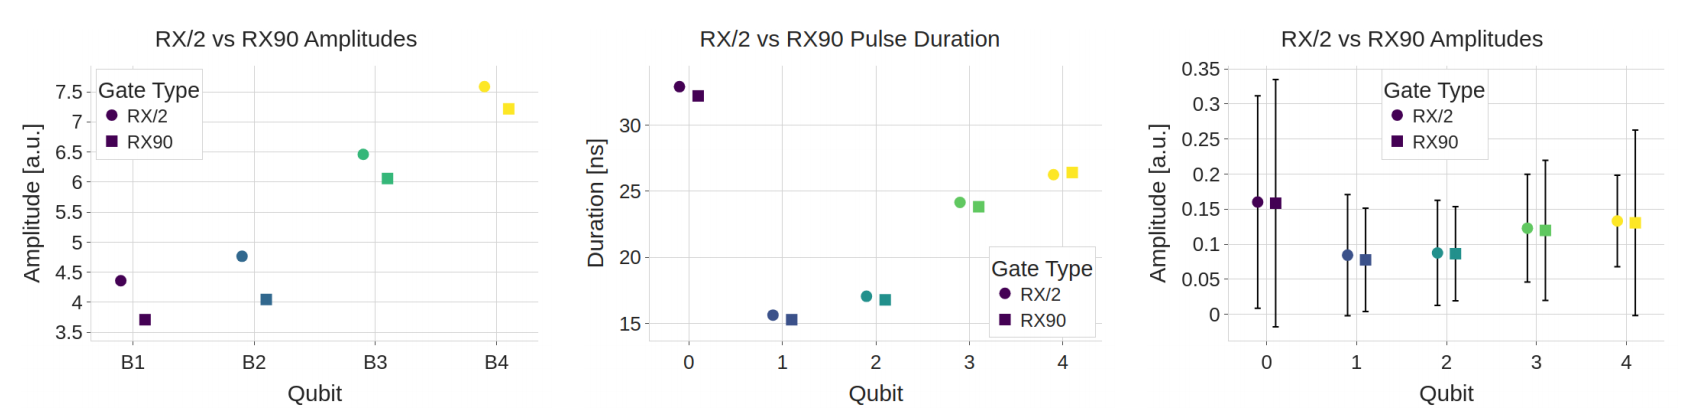
\includegraphics[width=\textwidth]{figures/RX90.png}
  \end{figure}
\end{frame}

\begin{frame}{Rabi amplitude experiment}
    \begin{figure}
    \centering
    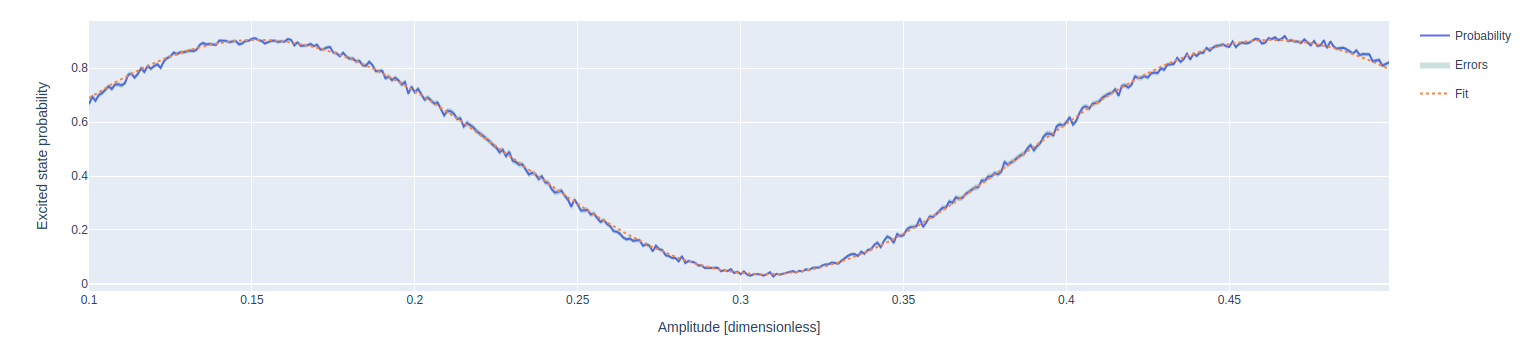
\includegraphics[width=\textwidth]{figures/B4.png}
    \vfill
    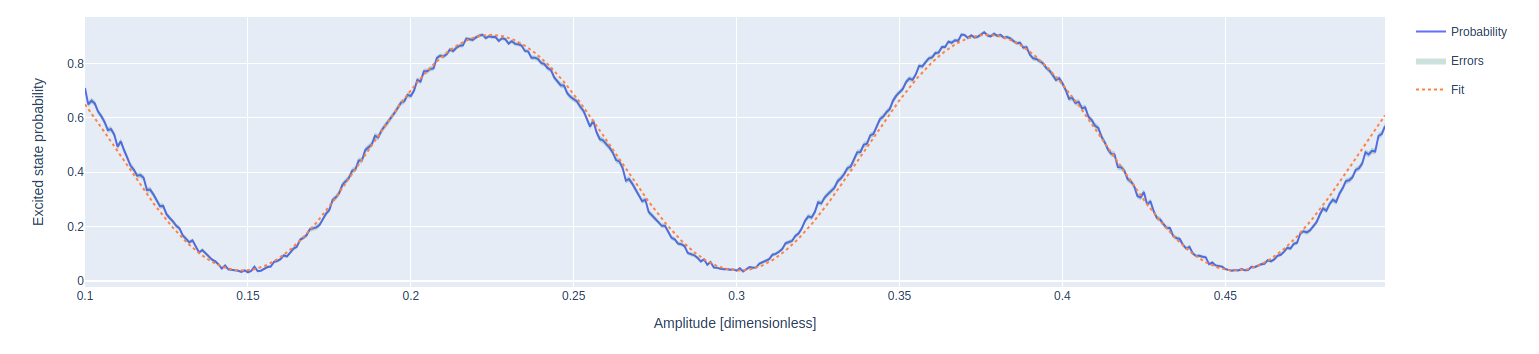
\includegraphics[width=\textwidth]{figures/B4_90.png}
  \end{figure}
\end{frame}


\subsection{Cryoscope}

\begin{frame}{Improving Qubit Control for Calibration}
  \onslide<1->{\textbf{Single qubit gates}:
  \begin{itemize}
    \item Qibo already implement many calibration routines for $R_X(\pi)$.
    \item We can try to reduce residual erros by adding directly calibrating $R_X(\pi/2)$.
  \end{itemize}
  Introduce support for $R_X(\pi/2)$ as native gate in Qibolab.\\
  \vspace*{1.em}
  \textbf{Two qubit gates}:}
  \begin{itemize}
    \item<2-> Two-qubit gates typically require bringing qubits into resonance.
    \item<3-> Frequency tuning is achieved via flux pulses applied to tunable qubits.
  \end{itemize}
  <4->Add Cryoscope portocol to improve control over flux pulses.
\end{frame}

\begin{frame}{Flux pulse reconstruction \hfill{\small[arXiv:1907.04818]}}
  \begin{columns}
    \begin{column}{0.4\textwidth}
      \centering
      \onslide<1->{Transmon frquency dependence on magnetic flux:
      \begin{equation*}
        f_q(\Phi_q) \approx \left( \sqrt{8E_J E_C \left| \cos\left(\pi \frac{\Phi_q}{\Phi_0}\right) \right|} \right).
      \end{equation*}\\}
      \vspace{1em}
      \onslide<4->{Detuning as function of the flux pulse:
      \begin{align*}
        \Delta f_q = &\frac{\varphi_{\tau+\Delta\tau}-\varphi_\tau}{2\pi} \approx \\
        &\frac{1}{\Delta \tau} \int_{\tau}^{\tau + \Delta \tau} \Delta f_q(\Phi_{q, \tau + \Delta \tau} (t)).
      \end{align*}}
    \end{column}
    \begin{column}{0.6\textwidth}
      \begin{figure}
        \centering
        \onslide<2->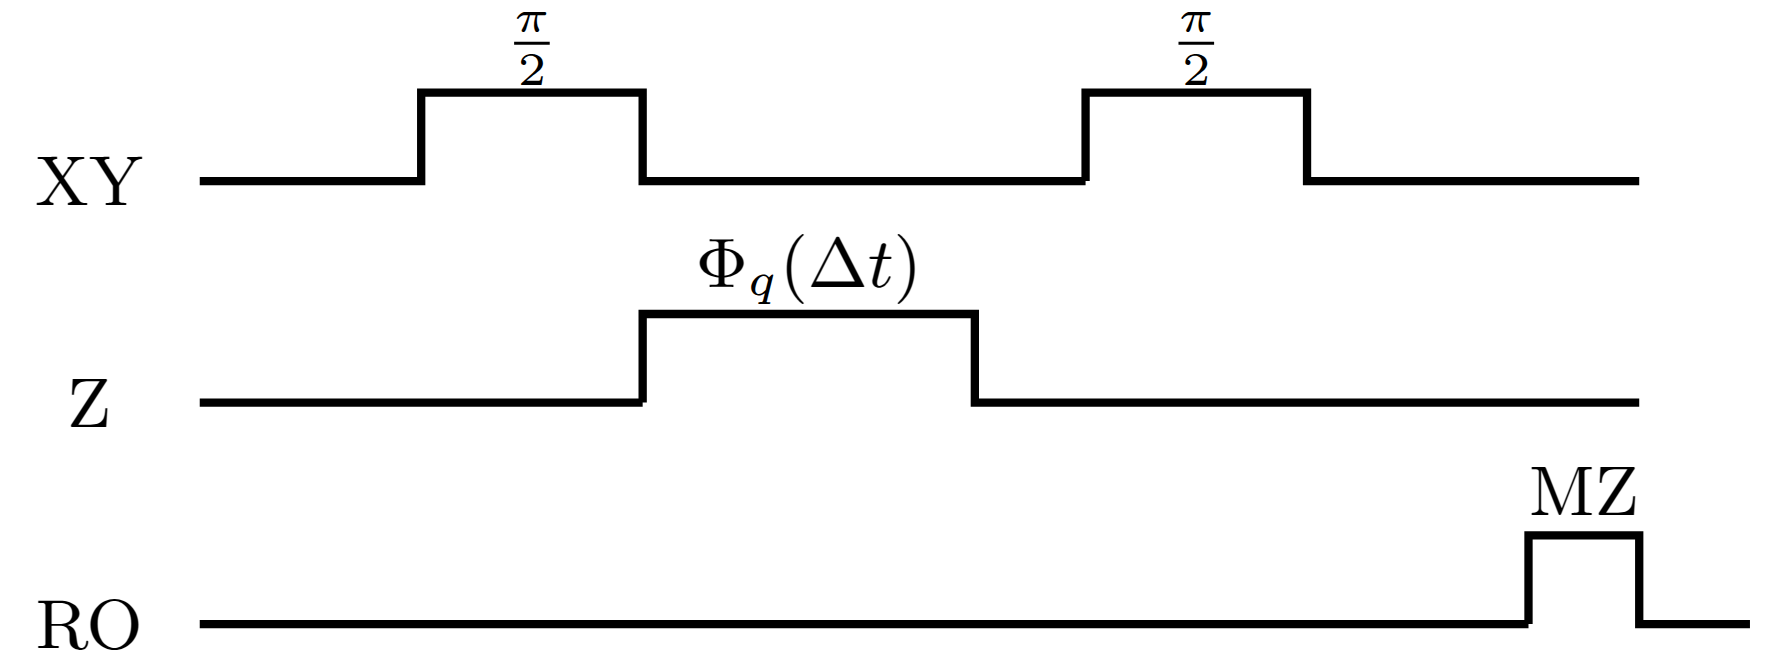
\includegraphics[width=0.85\textwidth]{figures/cryoscope_pulse.png}\\
        \vspace{3em}
        \onslide<3->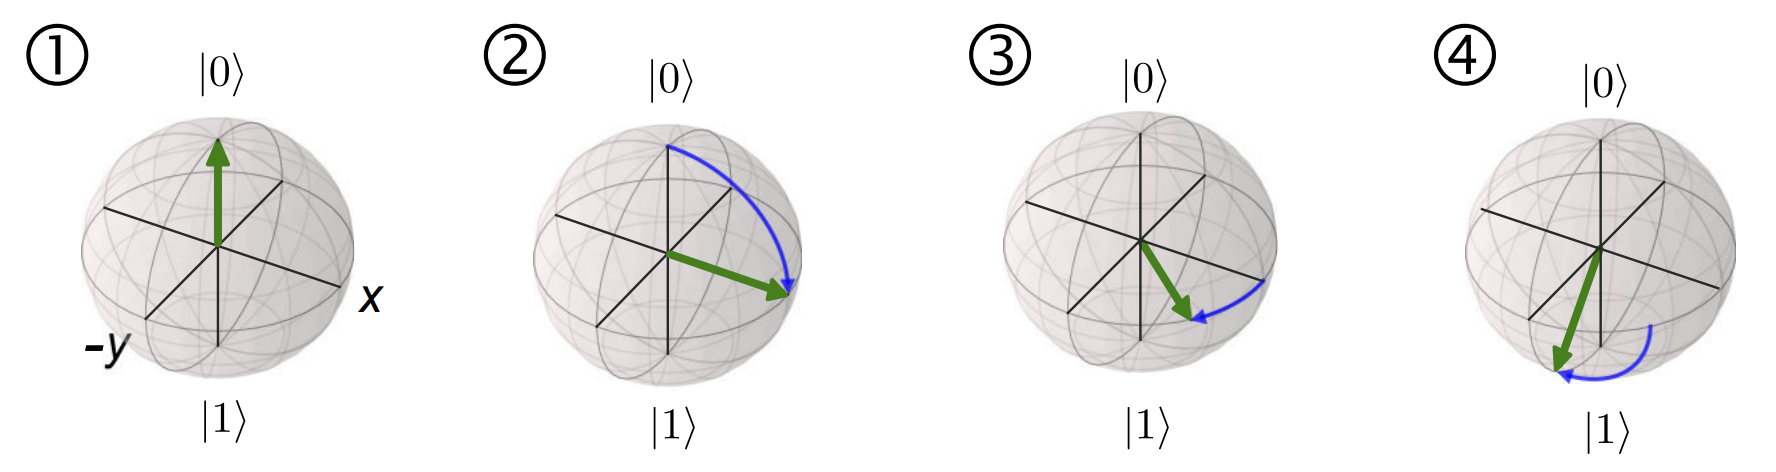
\includegraphics[width=0.85\textwidth]{figures/BlochEvolution.png}\\
        \onslide<3->{\tiny DOI: 10.1039/D2TC01258H}
      \end{figure}
    \end{column}
  \end{columns}
\end{frame}

\begin{frame}{Filter determination}
  \begin{enumerate}[leftmargin=*, label=\arabic*.]
    \item<1-> Determine exponential correction
    \item<2-> Obtain coefficients for the Infinite Impulse Response from exponential correction
    \item<3-> Determine Finite Impulse Response coefficients
    \item<4-> Obtain coefficients for real-time correction
  \end{enumerate}
\end{frame}

\begin{frame}{Filter determination}
  \begin{figure}
    \centering
    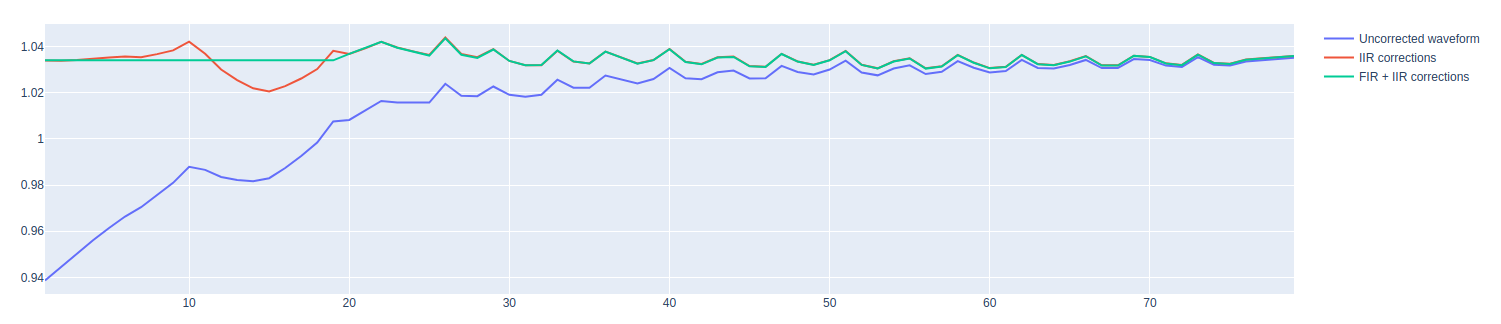
\includegraphics[width=\textwidth]{figures/B4_ringin.png}
  \end{figure}
  \vspace{0.5em}
  {\setbeamertemplate{enumerate items}[default]
    \begin{enumerate}[leftmargin=*, label=\arabic*.]
      \item Determine exponential correction
      \item Obtain coefficients for the Infinite Impulse Response from exponential correction
      \item Determine Finite Impulse Response coefficients
      \item Obtain coefficients for real-time correction
    \end{enumerate}}
\end{frame}

\begin{frame}{Impact of correction on chevron plots}
  \begin{figure}
    \centering
    \onslide<1->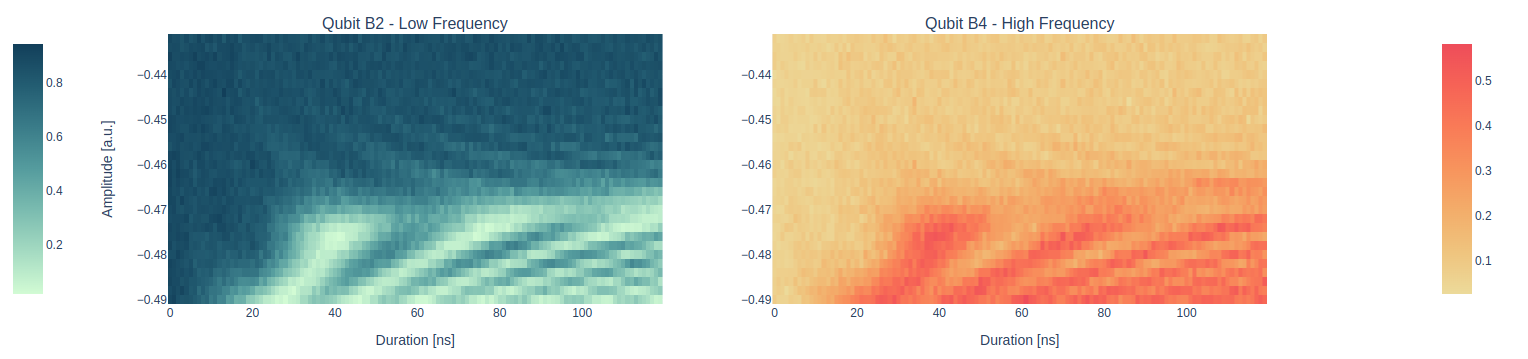
\includegraphics[width=\textwidth]{figures/B2B4_nofilter.png}
    \vfill
    \onslide<2->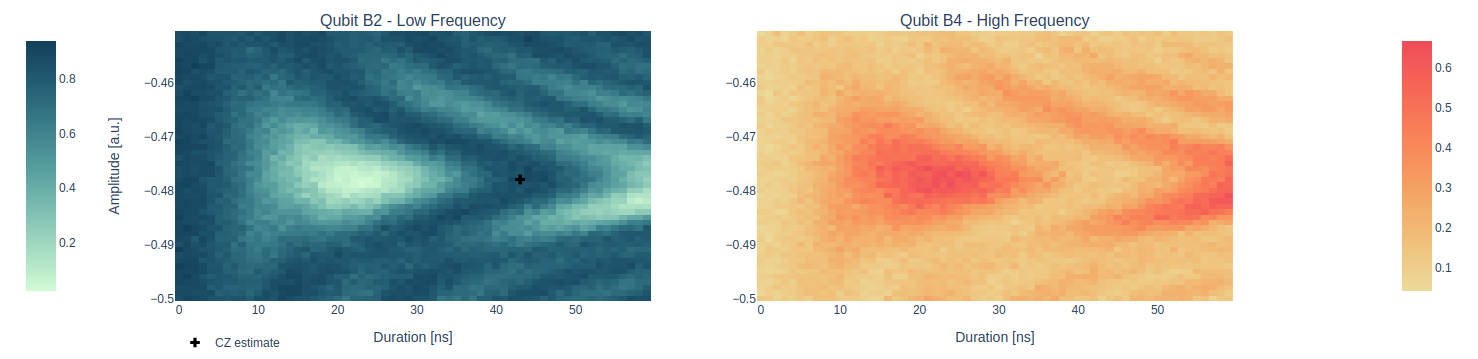
\includegraphics[width=\textwidth]{figures/B2B4.png}
  \end{figure}
\end{frame}

\begin{frame}{Cryoscope routine}
  \centering
  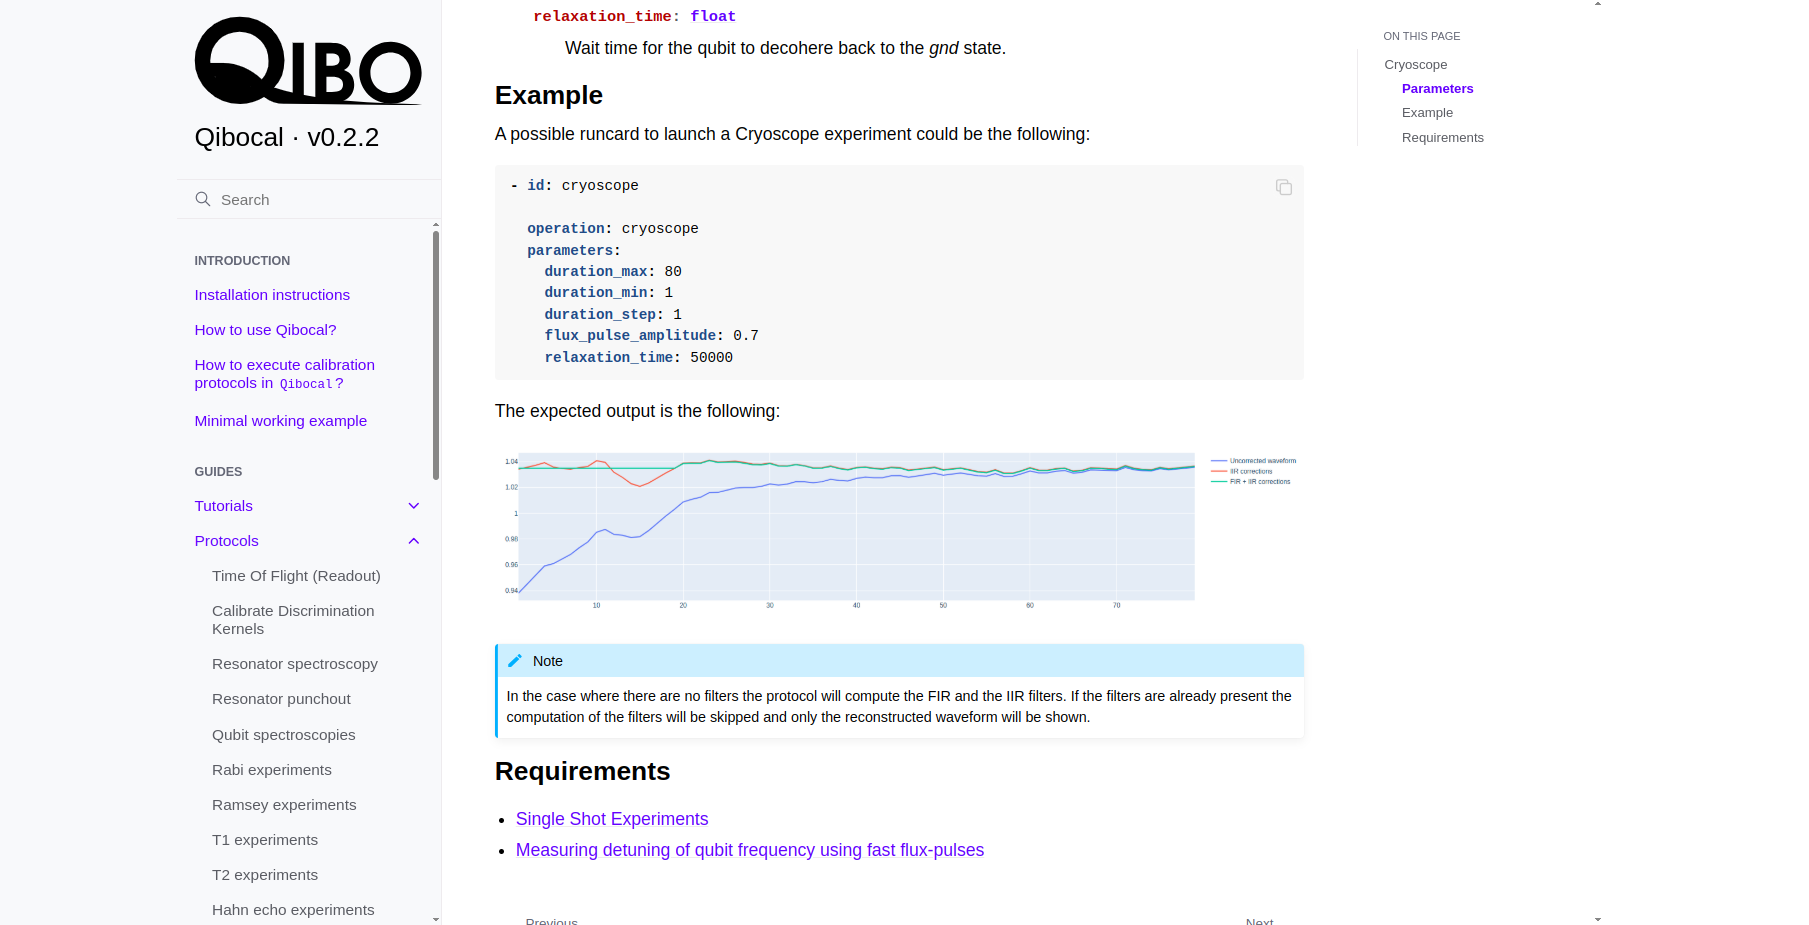
\includegraphics[height=\textheight]{figures/cryoscope_routine.png}
\end{frame}


\section{Conclusions \& Outlooks}

\begin{frame}{Gate recalibration by RB optimization}
  \begin{itemize}
    \item[\ding{51}] We can always find parameters configuration with average Clifford gate fidelity $> 99.5\%$.
    \item[\ding{51}] Does \textbf{not rely on manual tuning} by an operator.
    \item[\ding{55}] RB evaluation is \textbf{computationally expensive} ($\sim 30$ minutes).
    \item[\ding{55}] More stable methods (eg. Nelder-Mead) require many cost function evaluation.
    \item[\ding{55}] Parameters drift makes optimization unstable.
  \end{itemize}
  Possible future work: \textbf{optimize RB parameters} to allow a faster and more reliable optimization.
\end{frame}

\begin{frame}{Library additions}
  \begin{itemize}
    \item[\ding{51}] Extended Qibolab and Qibocal libraries to support \textbf{native $R_X(\pi/2)$ gates} with dedicated calibration routines.
    \item[\ding{51}] Implemented and added the \textbf{Cryoscope} calibration experiment to Qibocal library to correct flux-pulse distortions (average NMSE improvement $\sim 70\%$).
    \item[\ding{55}] Study long-time distortions of the flux-pulse.
  \end{itemize}
  Possible future extensions: 
  \begin{itemize}[label={\raisebox{0.2ex}{\tiny$\bullet$}}]
    \item Readout optimization protocols
    \item Active qubit reset schemes
    \item Implement leakage mitigation strategies
  \end{itemize}
\end{frame}

\begin{frame}[t,standout]
\Large
Thank you
\end{frame}

%%%%%%%%%%%%%%%%%%%%%%%%%%%%%%%%%%%%%%%%%%% BACKUP SLIDES %%%%%%%%%%%%%%%%%%%%%%%%%%%%%%%%%%%%%%%%%%%

\backupbegin
\appendix


\section*{Backup slides}

\begin{frame}{Qubit platforms}
  \begin{center}
      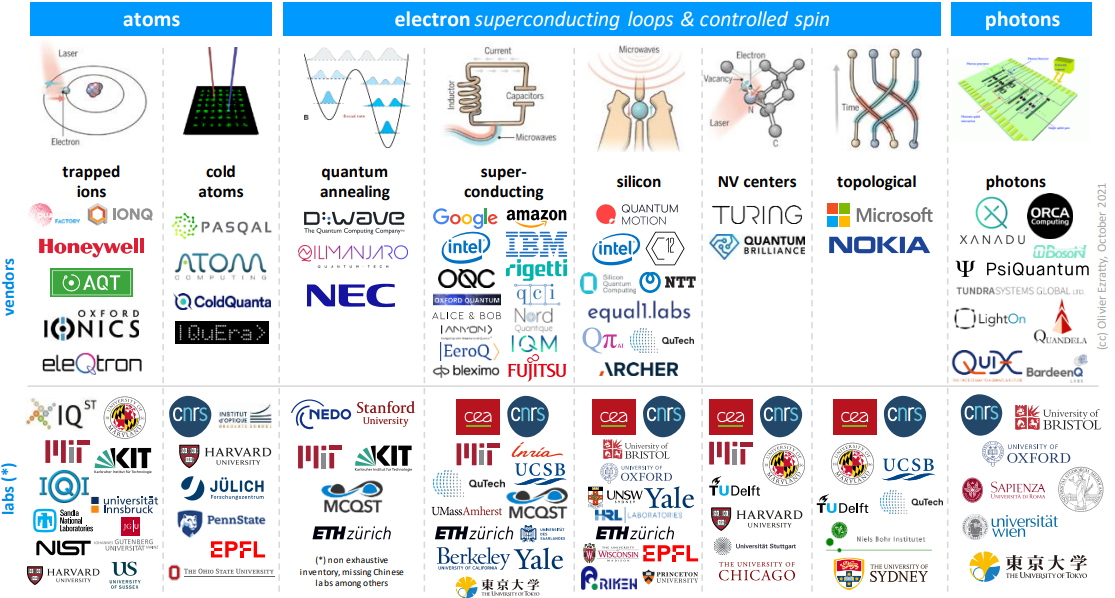
\includegraphics[height=0.82\textheight]{figures/platforms.png}
  \end{center}
\end{frame}

\begin{frame}{Calibration workflow \& assessment}
  \vbox to \textheight{ 
    \begin{minipage}[t]{\textwidth}
      \vspace{1.5em}
      \centering
      \begin{columns}
        \begin{column}{0.4\textwidth}
          Procedure:
          \setbeamertemplate{enumerate items}[default]
          \begin{enumerate}[leftmargin=*, label=\arabic*.]
            \item Resonator characterization
            \item Qubit characterization
            \item Gate calibration
            \item Gate set characterization
          \end{enumerate}
        \end{column}
      
        \begin{column}{0.4\textwidth}
          Metrics example:
          \begin{itemize}[label={\raisebox{0.2ex}{\tiny$\bullet$}}]
            \item readout \& assignment fidelity
            \item relaxation time $T_1$
            \item decoherence time $T_22$
            \item gate fidelity
          \end{itemize}   
        \end{column}
      \end{columns}
    \end{minipage}
    \vspace{1em}
  }
\end{frame}

\begin{frame}{Calibration workflow \& assessment}
  \vbox to \textheight{ 

    \begin{minipage}[t]{\textwidth}
      \centering
      \vspace{1.5em}
      \begin{columns}
        \begin{column}{0.4\textwidth}
          Main steps:
          \setbeamertemplate{enumerate items}[default]
          \begin{enumerate}[leftmargin=*, label=\arabic*.]
            \item Resonator characterization
            \item Qubit characterization
            \item Gate calibration
            \item Gate set characterization
          \end{enumerate}
        \end{column}
      
        \begin{column}{0.4\textwidth}
          Calibration quality metrics:
          \begin{itemize}[label={\raisebox{0.2ex}{\tiny$\bullet$}}]
            \item readout \& assignment fidelity
            \item relaxation time $T_1$
            \item decoherence time $T_22$
            \item gate fidelity
          \end{itemize}   
        \end{column}
      \end{columns}
    \end{minipage}
    \vspace{1em}


    \begin{minipage}[b]{\textwidth}
      \centering
      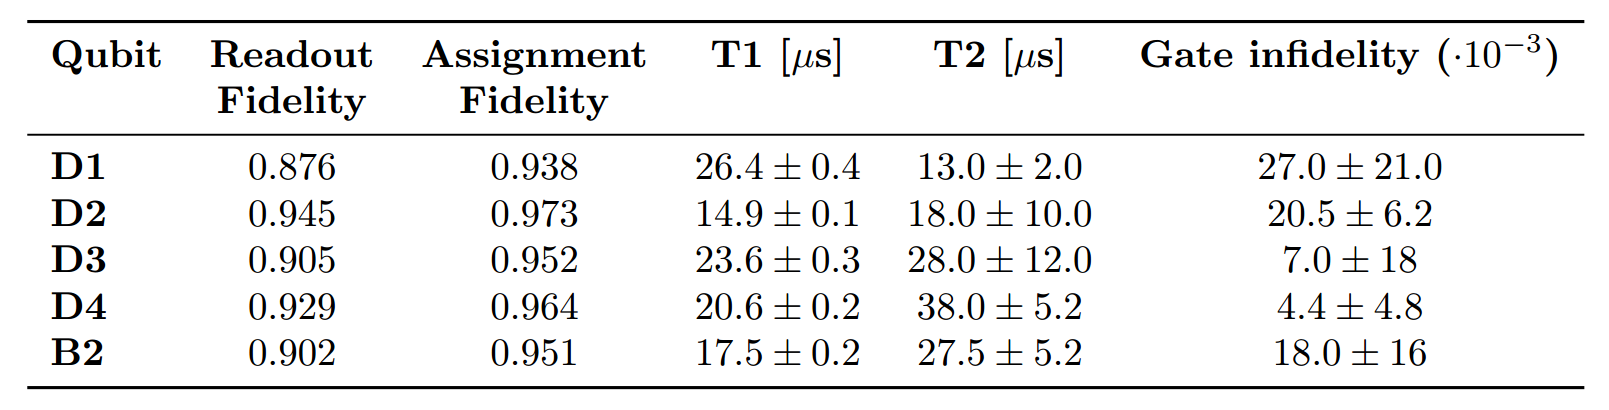
\includegraphics[height=0.4\textheight]{figures/cal_results.png}
    \end{minipage}
  }
\end{frame}



\begin{frame}{Clifford gates}
  \begin{columns}
    \begin{column}{0.4\textwidth}
      \begin{itemize}[label=\textbullet]
        \item Special subset of quantum gates that map Pauli operators to Pauli operators under conjugation
        \hspace{10mm}
        \item Clifford gates group is generated by $H$, $S$, ($CNOT$) gates
        \hspace{10mm}
        \item Quantum circuits that consist of only Clifford gates can be efficiently simulated with a classical computer (Gottesman–Knill theorem)
      \end{itemize}
    \end{column}
    \begin{column}{0.6\textwidth}
      \begin{figure}
        \centering
        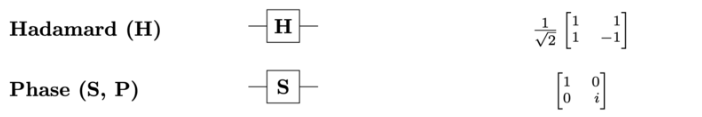
\includegraphics[width=\textwidth]{figures/HS.png}
        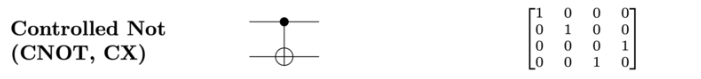
\includegraphics[width=\textwidth]{figures/CNOT.png}
        \vfill
      \end{figure}
    \end{column}
  \end{columns}
\end{frame}

\begin{frame}{RB optimization summary}
  \centering
  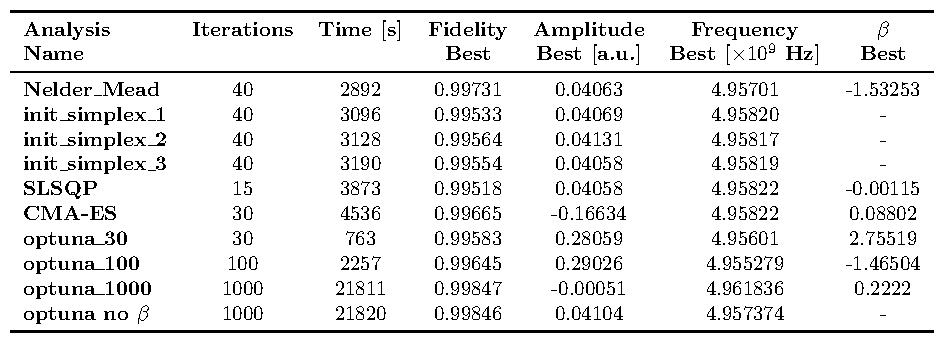
\includegraphics[width=\textwidth]{figures/recap_table.pdf}
\end{frame}


\begin{frame}{Filter determination details}
  \begin{center}
    Compensate distortion using a digital IIR filter based on an inverted exponential model
    \begin{equation*}
      s_{\text{corr}}(t) = \frac{s(t)}{g(1 - Ae^{-t/\tau})}
    \end{equation*}
    parameters $g$, $A$, and $\tau$ are estimated via least-squares minimization using \texttt{scipy.optimize}
  \end{center}

  \begin{figure}
    \centering
    \begin{subfigure}{0.48\textwidth}
      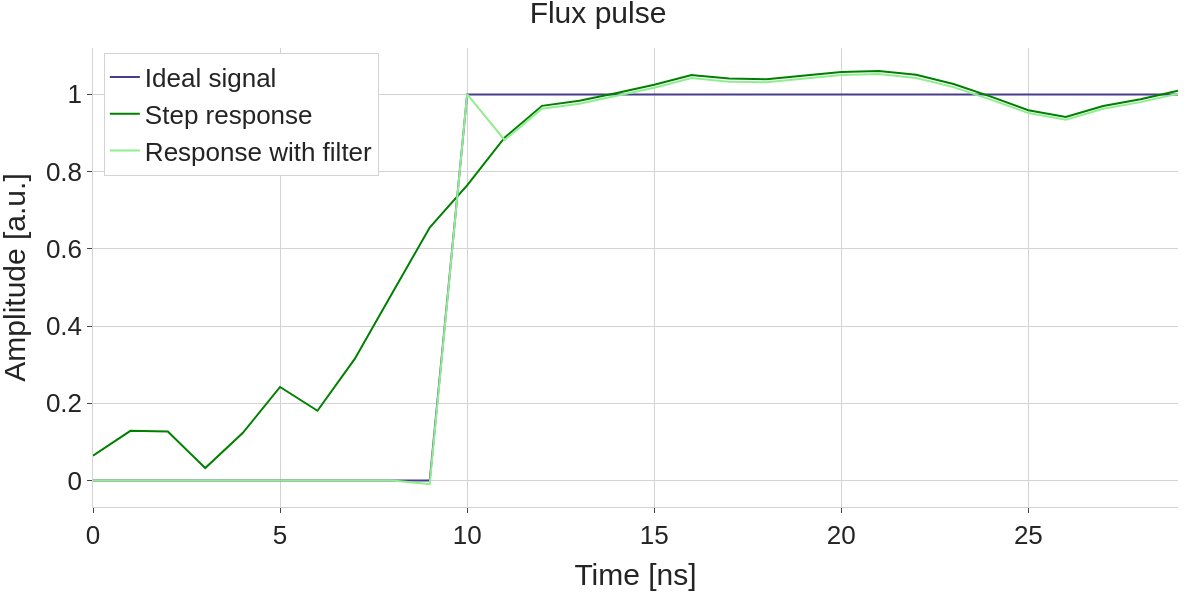
\includegraphics[width=\textwidth]{figures/step_inverse.png}
    \end{subfigure}
    \begin{subfigure}{0.48\textwidth}
      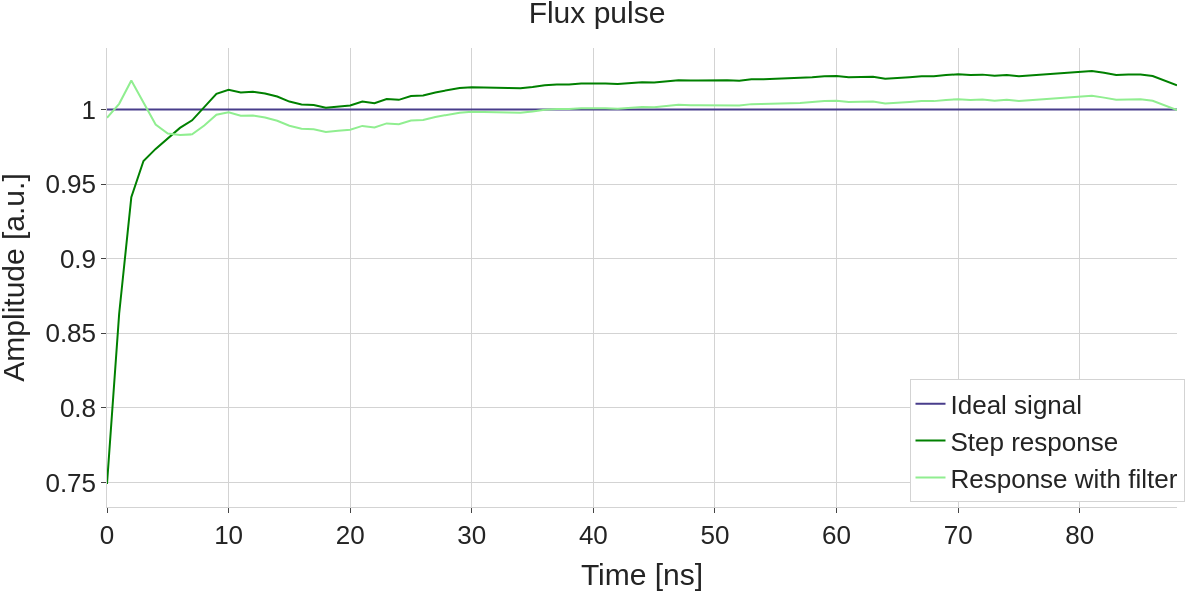
\includegraphics[width=\textwidth]{figures/inverse.png}
    \end{subfigure}
  \end{figure}

\end{frame}

\begin{frame}{Filter determination details}
  Digital IIR filter implemented in control hardware using discretized coefficients.
  \begin{equation*}
    \small
    a_0 y[n] = \sum_{i=0}^{N} b_i x[n - i] - \sum_{i=1}^{M} a_i y[n - i],
  \end{equation*}
  
  Filter coefficients derived from fitted parameters (1st order IIR):
  \begin{columns}
    \small
    \begin{column}{0.45\textwidth}
      \begin{align*}
        a_0 &= 1, \\
        a_1 &= -(1 - \alpha), \\
        b_0 &= 1 - k + k \alpha, \\
        b_1 &= -(1 - k)(1 - \alpha),
      \end{align*}
    \end{column}
    \begin{column}{0.55\textwidth}
      \centering
      where $  \alpha = 1 - \exp\left(-\frac{1}{f_s \cdot \tau (1 + A)}\right) $
      and
      \begin{equation*}
          k =
          \begin{cases}
          \frac{A}{(1 + A)(1 - \alpha)}, & \text{if } A < 0, \\
          \frac{A}{1 + A - \alpha}, & \text{if } A \geq 0,
          \end{cases}
      \end{equation*}
    \end{column}
  \end{columns}
  
  FIR filters:
  \begin{equation*}
    \small
        y[n] = \sum_{i=0}^{N} b_i x[n - i],
  \end{equation*}

  FIR filter coefficients are optimized using CMA-ES to minimize the average relative deviation between the FIR-filtered IIR-corrected signal and the ideal step response.

\end{frame}

\end{document}
